\documentclass[utf8x]{ctexart}
\usepackage{setspace}
\usepackage{url}
\onehalfspacing
\usepackage{amsmath,amssymb,amsfonts,amsthm,mathtools}
\usepackage[english]{babel}
\usepackage[T1]{fontenc}
\usepackage{lmodern}
\usepackage{dsfont}
\usepackage{bbm}
\usepackage[round]{natbib}
\usepackage{color} 
\usepackage[defaultlines=2,all]{nowidow}
\usepackage{caption}
\usepackage[labelformat=simple]{subcaption}
\usepackage{makecell}
\renewcommand\thesubfigure{(\alph{subfigure})}

\setlength\parindent{0pt}
\setlength{\parskip}{6pt plus 1pt minus 1pt}

\newcommand{\red}{\textcolor{red}}


\begin{document}

\begin{titlepage}
  \centering
  {\scshape\LARGE National Taiwan University \par}
  \vspace{1cm}
  {\scshape\Large Financial Technology \par}
  \vspace{2cm}
  {\huge\bfseries Project 2: Stock Price Prediction \par}
  \vspace{2cm}
  {\Large Lecturer:\\
    Che Lin (林澤) \par}
  \vspace{1cm}
  {\Large Author: Tadeo Hepperle (胡彬彬), Student ID: A11922105 \par}
  \vfill
  {\large \today\par}
\end{titlepage}


\tableofcontents

\cleardoublepage

\section{Introduction}

In this project historical data on the Apple Inc. stock is used to predict the stock's price on the next day. This is a regression task for which we are going to compare multiple methods:
\begin{itemize}
  \item A simple model always using the current day's Close price to predict the next day's Close price.
  \item A moving average model, that predicts the next day's Close price by a learned linear combination of the past 30 Close prices.
  \item An RNN Cell with one layer
  \item An LSTM Cell with one layer
  \item A GRU Cell with one layer
\end{itemize}

\subsection{Description of the data}

The dataset contains various technical features concerning the Apple Inc. stock price in the time interval between 2011/01/03 and 201/12/31. There is a total of 754 data points.
For each data point the following 6 features are available:
\begin{itemize}
  \item Open - price of the stock when markets opened
  \item High - highest price of the stock on that day
  \item Low - lowest price of the stock on that day
  \item Close - price of the stock when markets closed
  \item Volume - the total volume of the stock traded
  \item Adjusted Close - stock's value after accounting for any corporate actions
\end{itemize}

In addition to these inherent features, 5 other features were computed:
\begin{itemize}
  \item MA10 - 10 day moving average
  \item MA30 - 30 day moving average
  \item K - from the KD-indicator line chart
  \item D - from the KD-indicator line chart
  \item Weekday - one hot encoded into 7 different binary features
\end{itemize}

The data points are continous without gaps except for weekends and other days where the stock market is closed.
For method selection and model evaluation the data was split into train, validation and test sets:
\begin{itemize}
  \item Train set - stock price from 2011/01/01 - 2012/12/31
  \item Validation set - stock price from 2013/01/01 - 2013/06/30
  \item Test set - stock price from 2013/07/01 - 2013/12/30
\end{itemize}


\subsection{Description of methods}

The methods used are briefly described in the following sections to provide a deeper understanding.

\subsubsection{Last Value Model}

The simplest model to predict the next day's Close price is to just use the current day's Close price as the prediction. This model does not need any training and can be understood as a baseline model other models can be compared to in terms of their train and test loss.

\subsubsection{Moving Average Model}

A moving average in it's more general definition is a linear combination of the values of a subsequence of a sequence. In this model we want to form a linear combination of the past 30 Close values to predict the next Close price. For this we need to learn 30 weights.

\subsubsection{Recurrent Neural Network}

The recurrent neural network (RNN) is specified by 2 parameters: $input\_size$ and $hidden\_size$. In this project we always just use an RNN with 1 layer. The RNN learns over a period of $time\_steps = 30$ iterations. In each iteration, an input vector of size $input\_size$ and a hidden state vector of size $hidden\_size$ are concatinated into a combined vector which is fed through a ReLU-activated linear layer to produce the hidden state for the next iteration. In the initial iteration the hidden state is a zero-vector. After the $time\_steps$ iterations of this process, the hidden state is mapped by a linear layer to a single scalar value (the Close price we want to predict).
Mini-batch gradient descent is used to train such an RNN.

\subsubsection{LSTM}

LSTM stands for long short-term memory. The LSTM tries to improve on the RNN by using a cell state in addition to the hidden state, which is also a vector of $hidden\_size$. while the hidden state represents a short term memory because the gradients deteriorate over time, the cell state is connected via constant gradient flow and can store information for much longer.

\begin{math}
  \begin{aligned}f_{t}            & =\sigma _{g}(W_{f}x_{t}+U_{f}h_{t-1}+b_{f})     \\
               i_{t}            & =\sigma _{g}(W_{i}x_{t}+U_{i}h_{t-1}+b_{i})     \\
               o_{t}            & =\sigma _{g}(W_{o}x_{t}+U_{o}h_{t-1}+b_{o})     \\
               {\tilde {c}}_{t} & =\sigma _{c}(W_{c}x_{t}+U_{c}h_{t-1}+b_{c})     \\
               c_{t}            & =f_{t}\odot c_{t-1}+i_{t}\odot {\tilde {c}}_{t} \\
               h_{t}            & =o_{t}\odot \sigma _{h}(c_{t})
  \end{aligned}
\end{math}

in the equation abobe $x_t$ stands for the input feature vector at a given time $t$ starting from $t = 1$ up to $t = 30$ in our case. $h_t$ represents the hidden state, while $c_t$ is the cell state. In each iteration of the forward pass the formulas above are applied, to generate a new $h_t$ and $c_t$ until finally $h_{30}$ is mapped by a linear layer to a single scalar: the predicted Close value of the next day.

In theory, one could have multiple layers in each iteration, we will just use 1-layer LSTMs and GRUs in this project.

\subsubsection{GRU}

GRU stands for gated recurrent unit. In comparison to the LSTM it lacks the input/update gate and the cell state but has been found to produce similar results at a lower computational cost in many applications. In each forward pass the following formulas are applied to get from the input $x_t$ and the hidden state $h_t$ to the next hidden state:


\begin{math}
  \begin{aligned}z_{t}          & =\sigma _{g}(W_{z}x_{t}+U_{z}h_{t-1}+b_{z})            \\
               r_{t}          & =\sigma _{g}(W_{r}x_{t}+U_{r}h_{t-1}+b_{r})            \\
               {\hat {h}}_{t} & =\phi _{h}(W_{h}x_{t}+U_{h}(r_{t}\odot h_{t-1})+b_{h}) \\
               h_{t}          & =z_{t}\odot {\hat {h}}_{t}+(1-z_{t})\odot h_{t-1}\end{aligned}
\end{math}

\section{Results}

First we will provide descriptive statistics and graphics of the dataset before moving on to compare the regression methods with each other.

\subsection{Descriptive Statistics}

The price of the Apple Inc. stock fluctuated between \$67.9 and \$134.1 in the given time frame. A volume between \$800.000 and \$15.000.000 was traded every active day.
The 3 charts in Figure~\ref{fig:candles} display the price development, traded volume and KD-line in the entire timeframe of almost 2 years.

In the topmost candle-chart the blue line represents the 10-Day moving average, while the orange line is the 30-Day moving average.

The bottom chart shows the K (blue line) and D (orange line) statistics, both common technical indicators.

\label{fig:candles}
\begin{figure}[p]
  \vspace*{-2cm}
  \makebox[\linewidth]{
    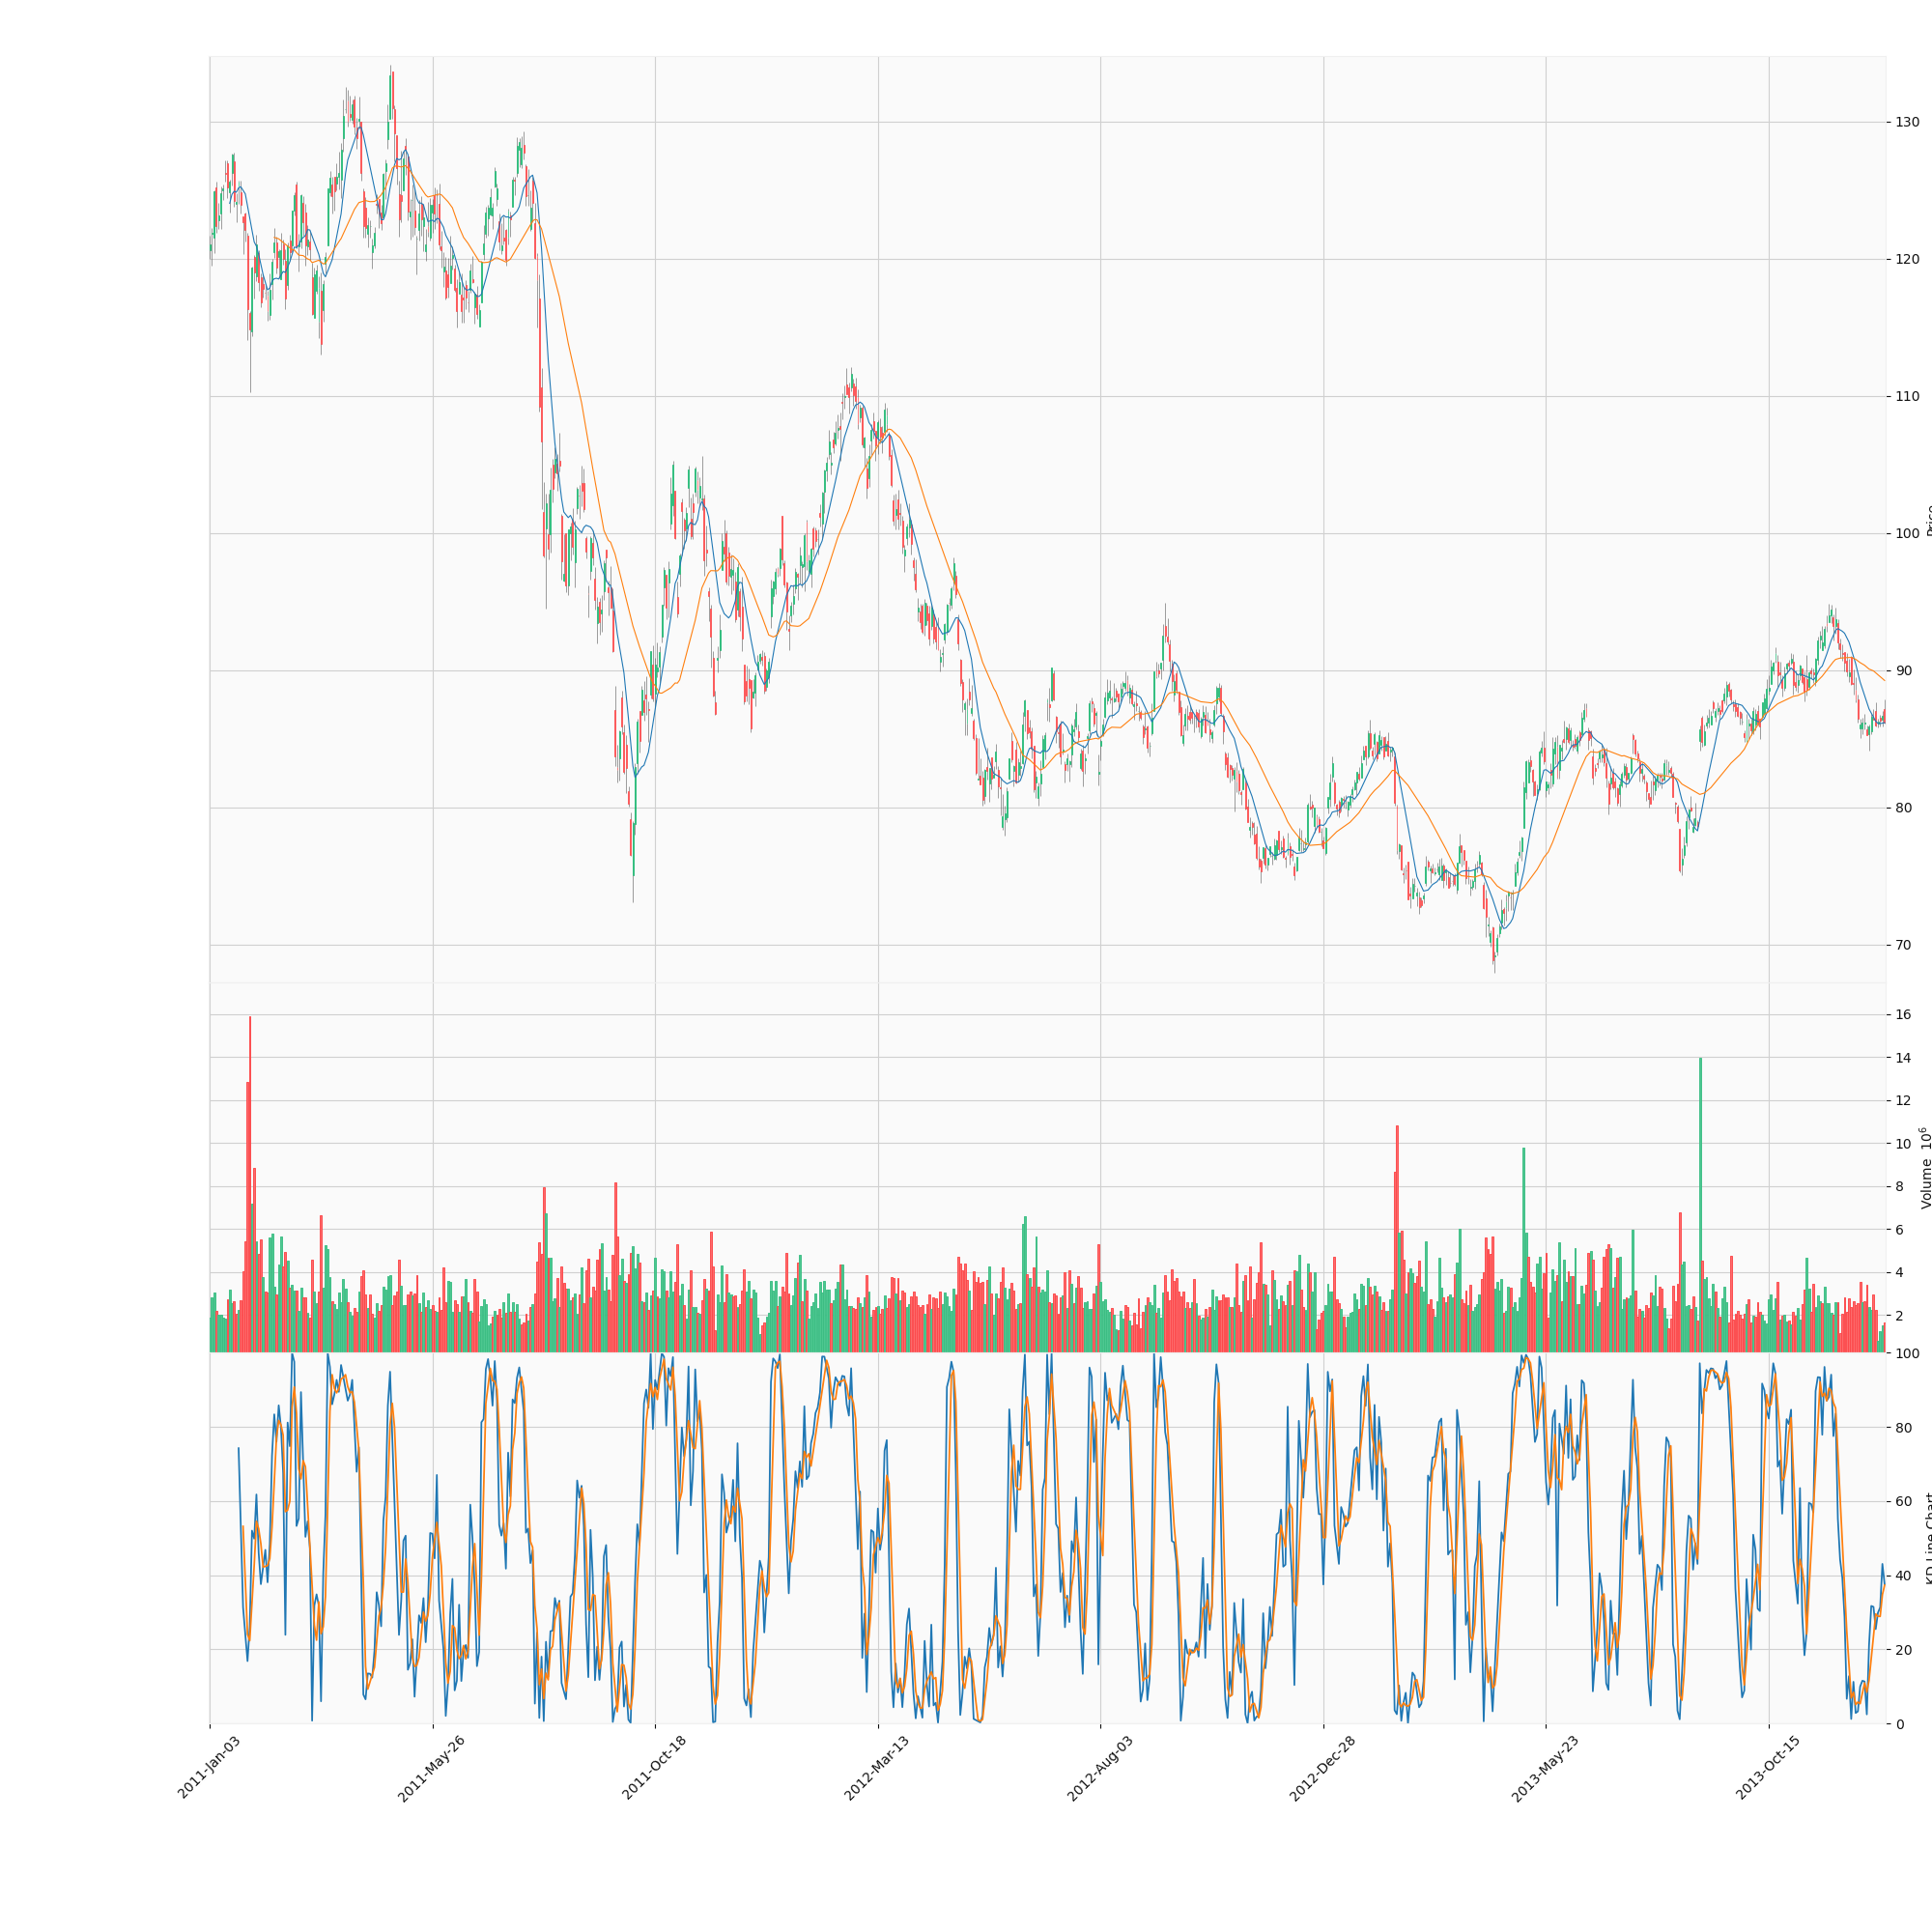
\includegraphics[width=1.3\linewidth]{../images/candles_KD_volume.png}
  }
  \caption{Sequence diagram}
\end{figure}

In the candlestick chart, red sticks represent days where the stockprice decreased, green sticks indicate an increase in the price. The same color coding is also used for the bars of the volume chart. We see that the proportion of increasing days is roughly equal to decreasing days. The KD-chart oscillator curve looks mainly random, we cannot observe a strong pattern from it.
Before applying any prediction model the features and labels (Close price of the next day) were min-max normalized to a range between 0 and 1. The weekdays were computed from the date and one-hot-encoded.

\subsection{Last Value Model}

As a  baseline for all further learning we need to know how well we can predict the next Close price with a very simple model: What if we just take the last day's Close price as the prediction?
Such a model yields results on the 3 data set slices like displayed in Table~\ref{tab:last_value_model} and gives price predictions like shown in Figure~\ref{fig:last_value_model}.

\begin{figure}[htb]
  \centering
  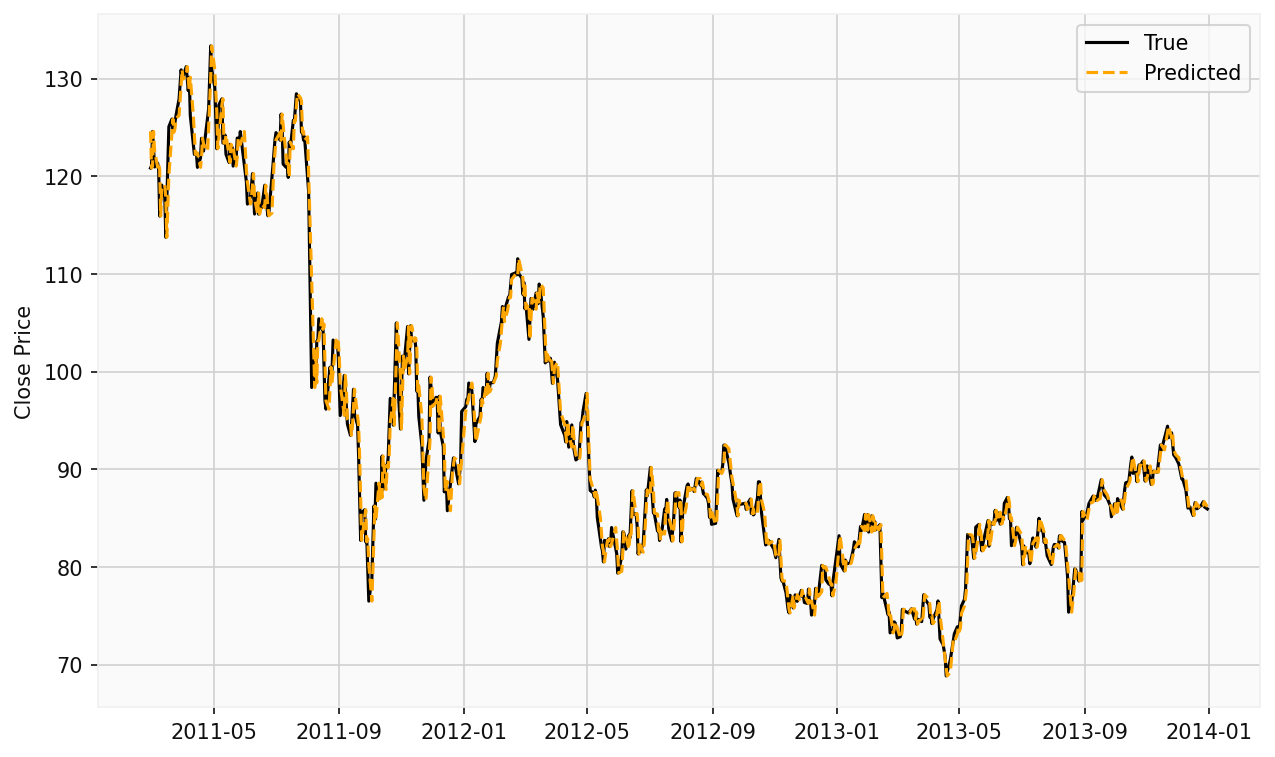
\includegraphics[width=\textwidth]{../images/last_value_model.png}
  \caption{Predictions of the Last Value Model}
  \label{fig:last_value_model}
\end{figure}

\begin{table}[ht]
  \centering
  \caption{MSE of the Last Value Model on train, validation and test set}
  \label{tab:last_value_model}
  \begin{tabular}{c|ccc}
        & Train set & Validation set & Test set \\
    \hline
    MSE & 0.00102   & 0.00035        & 0.00028  \\
  \end{tabular}
\end{table}

It will be compared to other models below.
The MSE is a popular loss function for regression tasks and is defined as

\[ MSE = \frac{1}{n} \sum_i{(y_i - \hat{y}_i)^2}\]

where $y_i$ are the true values and $\hat{y}_i$ are the predictions.

\subsection{Moving Average Model}

Pytorch was used to train a neural network with 1 linaer layer that models the next Close Price as a Moving Average of the last 30 days with variable weights. The weights were initialized to resemble the Last Value model at first, s.t. $w = [0,0,\dots,0,1]$ and $Card(w) = 30$. The validation set was used to determine when to stop the training. There was no visible overfitting on the validation set, that's why it was run for 800 epochs, with batchsize 32 and a learning rate of 0.001 and showed good convergence.

The final moving average coefficients resemble a lot of similarity to the Last Value Model: The vector looks a lot like this: [..., 0.256, 0.796], where all preceding values are smaller than 0.120 in absolute value. This means that still the most recent value has the greatest weight in predicting the next Close value.
Loss curve and predictions on the test set can be viewed in Figure~\ref{fig:losses} and Figure~\ref{fig:predictions}.

Loss statistics in terms of MSE can be viewed in Table~\ref{tab:comparison}.

\subsection{RNN, LSTM and GRU}

for the RNN, LSTM and GRU via hyperparameter tuning the following paramters were deemed best:
\begin{itemize}
  \item $epochs = 50$ (RNN, GRU) | $100$ (for LSTM) - after 50 epochs there was visible overfitting as the validation test error began to rise again. The LSTM took a bit longer until the overfitting zone was hit.
  \item $learning\_rate = 0.001$ - a larger learning rate converged faster but the MSE did not go as low and jumped around more. Smaller learning rates increased the number of EPOCHS needed without yielding better results.
  \item $size\_of\_hidden\_state = 64$ - seemed appropriate, but did not affect the outcome too much (32 and 128 were tried as well).
  \item $size\_of\_input = 17$ - all available features were used, 7 of which are the one-hot-encoded weekdays, other than that: $Close$, $Open$, $Low$, $High$, $Adj.Close$, $Volume$, $MA10$, $MA30$, $K$, $D$.
  \item $batch\_size = 32 $ - gave good results.
\end{itemize}

Notice, that the paramters were the same for all 3 models (RNN, LSTM, GRU), except for the $epochs = 100$ in the LSTM. The cell state size in the LSTM equals the hidden size (64).
All models used a time frame of 30 days for the predictions. Figure~\ref{fig:losses} shows how the loss developed during training. Sadly because the first 2-3 Epochs had a quite dramatic loss, the following continous decline in the MSE is not visible too well. Notice that the MSE is related to the normalized stock price values, that range from 0 to 1. The real MSE of the price in US-dollars is likely around $x$ times as high, where
\[ x \approx (max(Close) - min(Close))^2 \approx (134.1 - 67.9)^2 \approx 4382 \]


\begin{figure}[htb]
  \centering
  \begin{subfigure}[b]{0.48\textwidth}
    \centering
    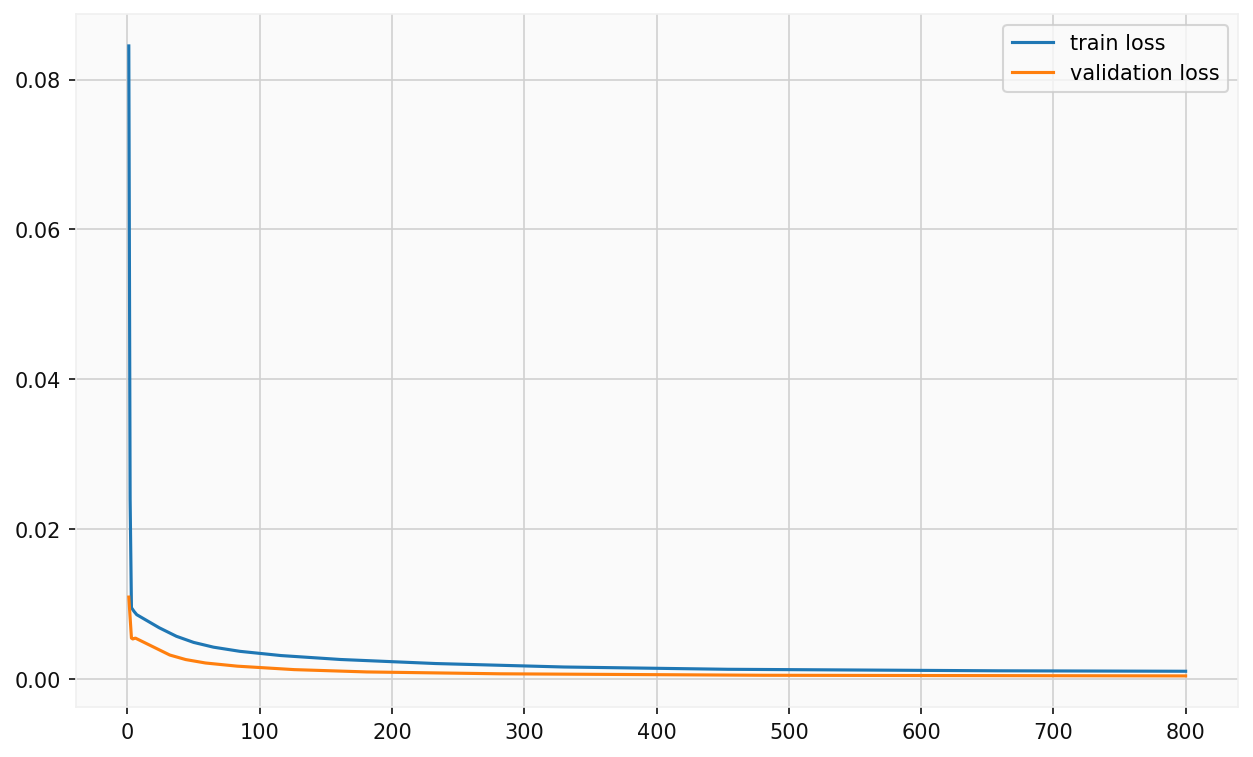
\includegraphics[width=\textwidth]{../images/ma_losses.png}
    \caption{Moving Average Model}
    \label{fig:ma_losses}
  \end{subfigure}
  \begin{subfigure}[b]{0.48\textwidth}
    \centering
    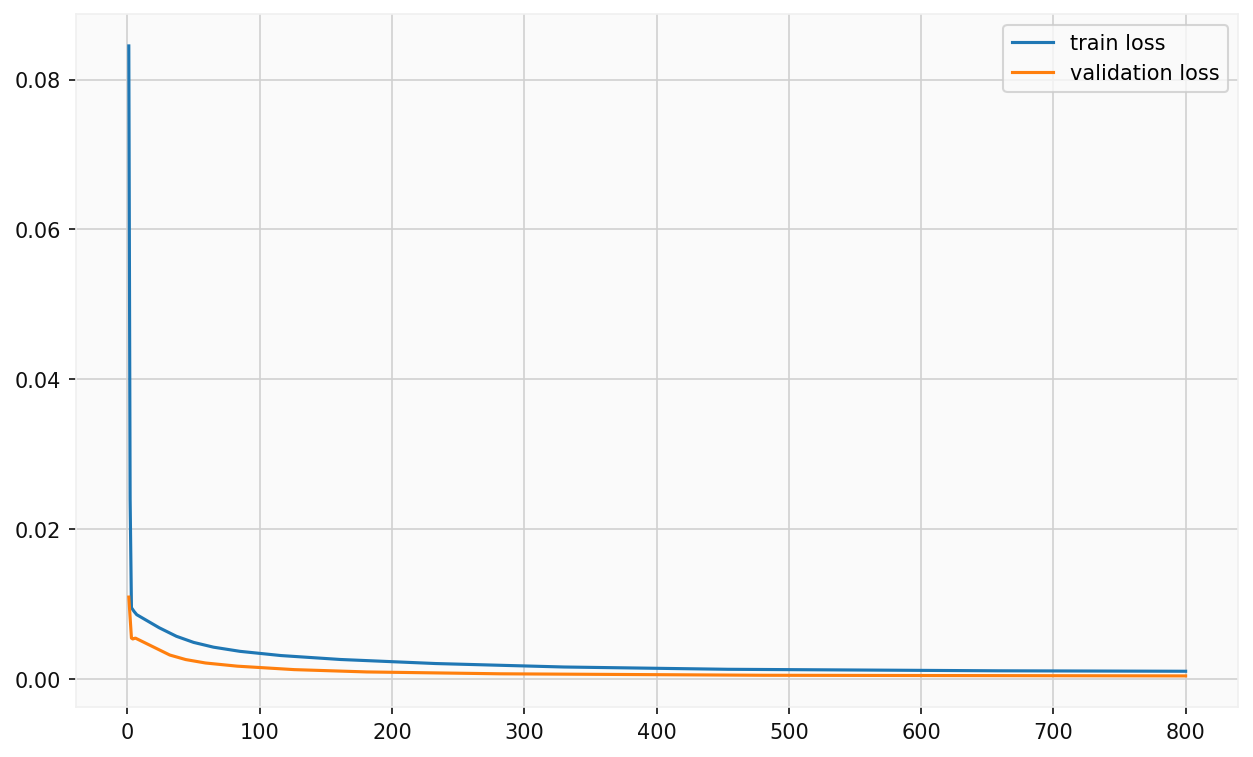
\includegraphics[width=\textwidth]{../images/rnn_losses.png}
    \caption{RNN}
    \label{fig:rnn_loss}
  \end{subfigure}
  \begin{subfigure}[b]{0.48\textwidth}
    \centering
    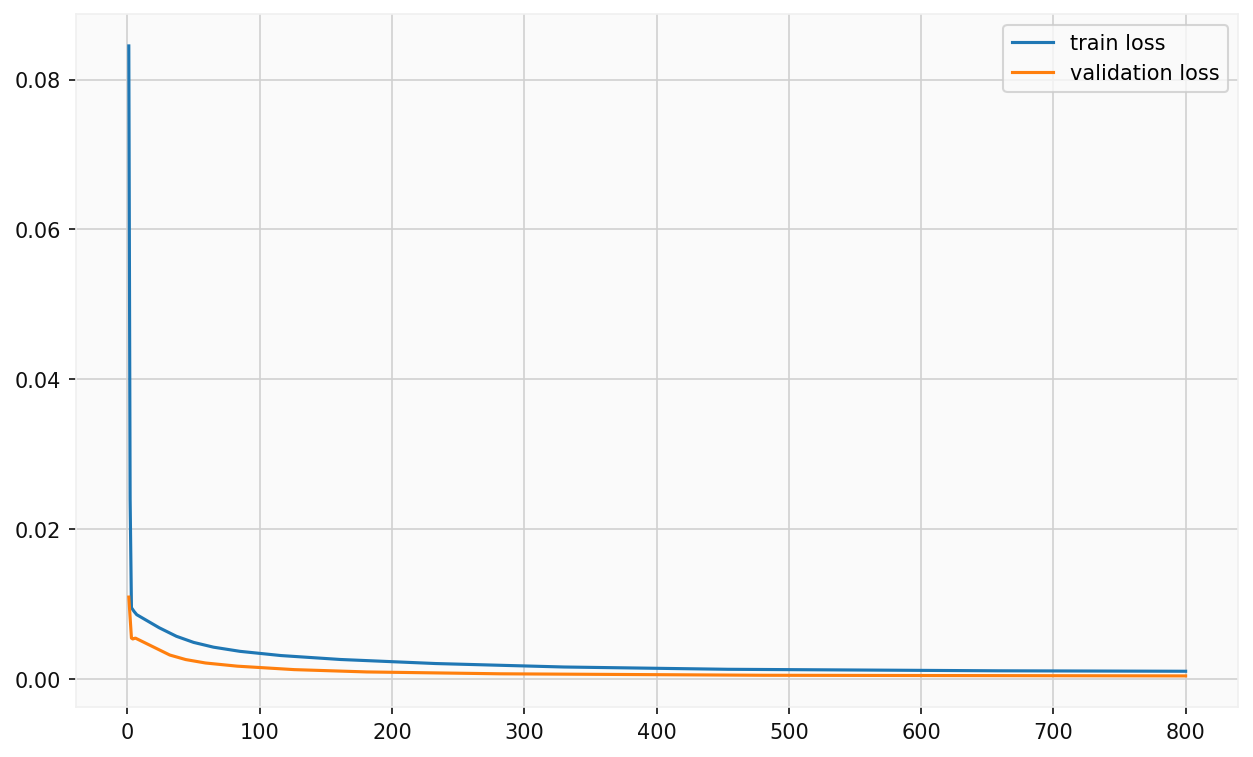
\includegraphics[width=\textwidth]{../images/lstm_losses.png}
    \caption{LSTM}
    \label{fig:lstm_loss}
  \end{subfigure}
  \begin{subfigure}[b]{0.48\textwidth}
    \centering
    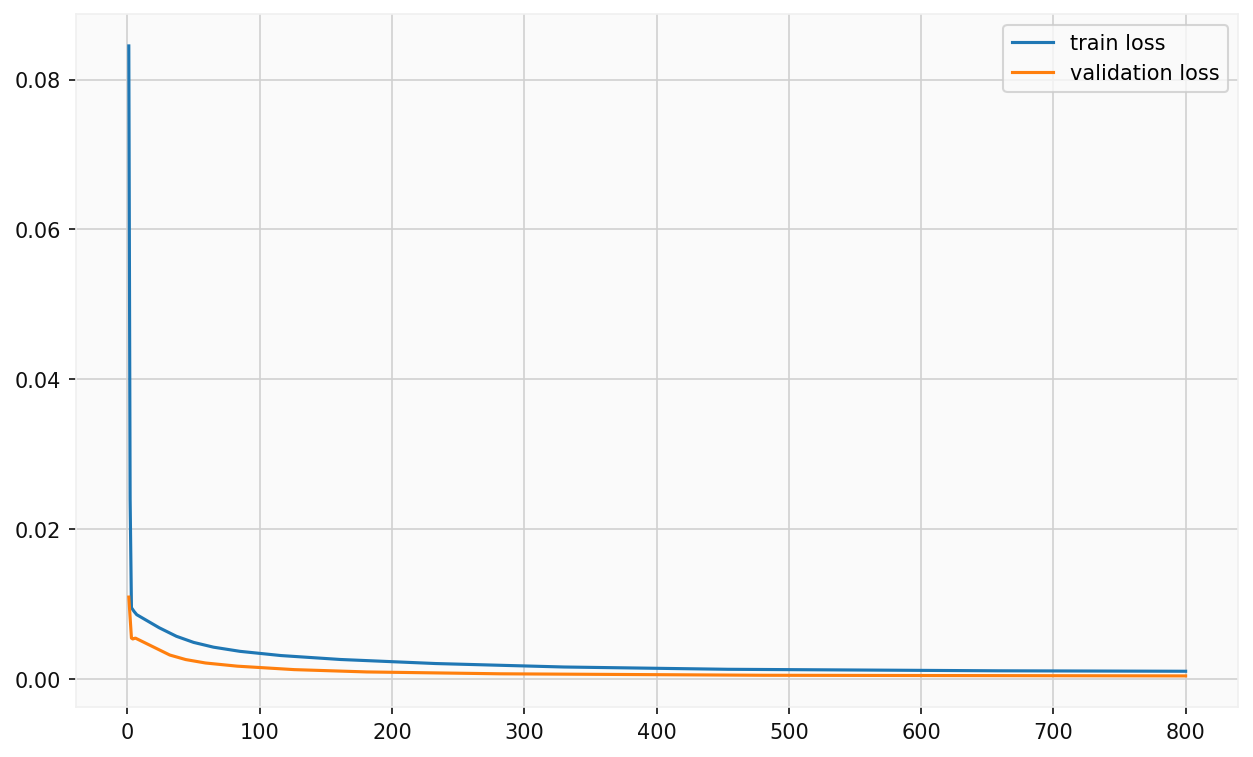
\includegraphics[width=\textwidth]{../images/gru_losses.png}
    \caption{GRU}
    \label{fig:gru_loss}
  \end{subfigure}
  \caption{Train and validation set losses (MSE) of Moving Average Model, RNN, LSTM and GRU throughout training}
  \label{fig:losses}
\end{figure}


Figure~\ref{fig:predictions} shows how the 4 different models perform on predicting unseen values in the test set given the last 30 observations. As we can see, all of them somewhat seem to have learned the representation of the data and make use of it. But if we look at the values in Table~\ref{tab:comparison} we see that all of the models perform similarly but none of them outperforms the simple Last Value Model. In experimentations with more epochs it was possible to push the train error down to as little as 0.00007 for RNN, GRU and LSTM, however at the cost of increasing validation and test error. This is not desirable and shows overfitting. Thus given the limited data, none of the models seems to be actually a good choice for the prediction of the values in the test set. In fact the MSE of the neural network models seems to be almost two times as high as the MSE of the baseline Last Value Model on the test set as the column $"Comparison"$ in Table~\ref{tab:comparison} shows.


\begin{table}[ht]
  \centering
  \caption{MSE of the Last Value Model on train, valaidation and test set}
  \label{tab:comparison}
  \begin{tabular}{c|cccc}
    MSE                  & Train   & Validation & Test    & Comparison \\
    \hline
    Last Value Model     & 0.00102 & 0.00035    & 0.00028 & 100\%      \\
    Moving Average Model & 0.00103 & 0.00042    & 0.00034 & 121\%      \\
    RNN                  & 0.00106 & 0.00087    & 0.00055 & 196\%      \\
    LSTM                 & 0.00112 & 0.00058    & 0.00050 & 179\%      \\
    GRU                  & 0.00118 & 0.00050    & 0.00050 & 179\%      \\
  \end{tabular}
\end{table}

RNN, LSTM and GRU show similar performance on this task. The observed MSE rates are not different enough to provide evidence that one would be better than another. Also the lower test MSE of GRU and LSTM might be more due to randomness and is not wildly different from the pure RNN.



\begin{figure}[htb]
  \centering
  \begin{subfigure}[b]{0.48\textwidth}
    \centering
    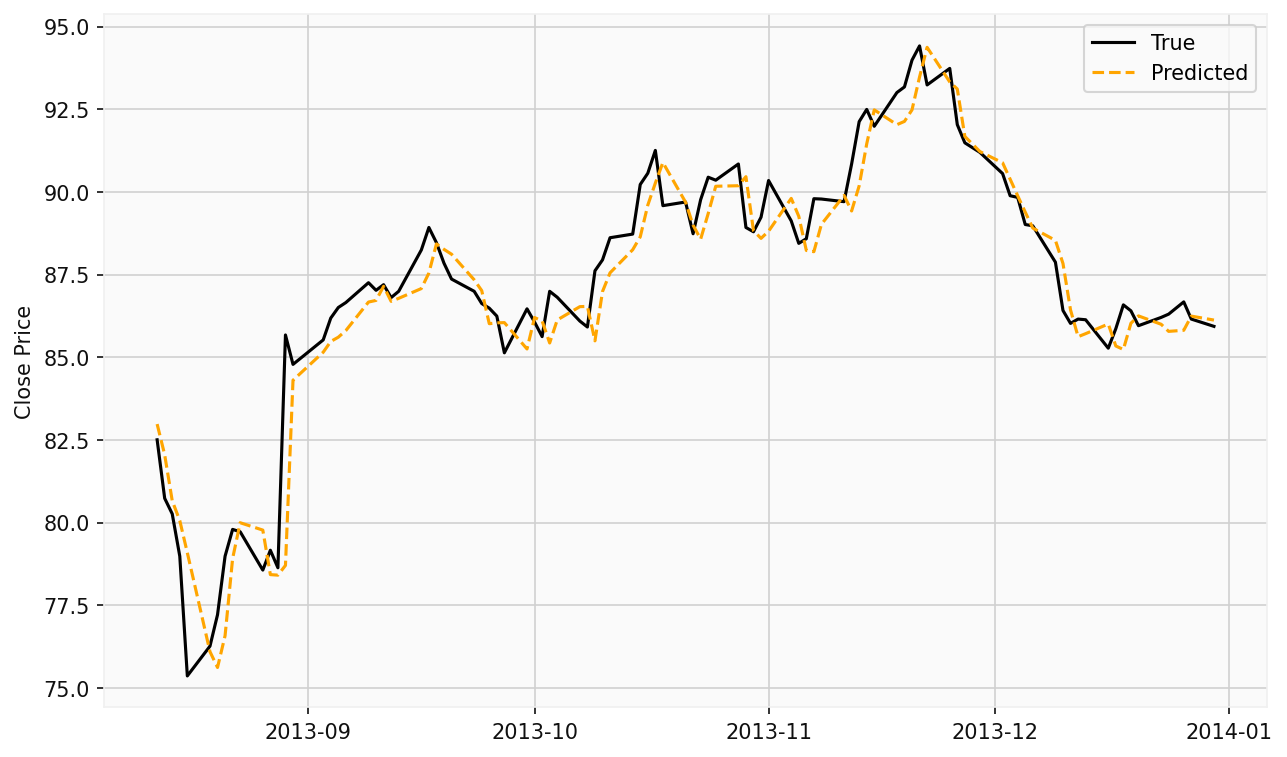
\includegraphics[width=\textwidth]{../images/ma_prediction.png}
    \caption{Moving Average Model}
    \label{fig:ma_prediction}
  \end{subfigure}
  \begin{subfigure}[b]{0.48\textwidth}
    \centering
    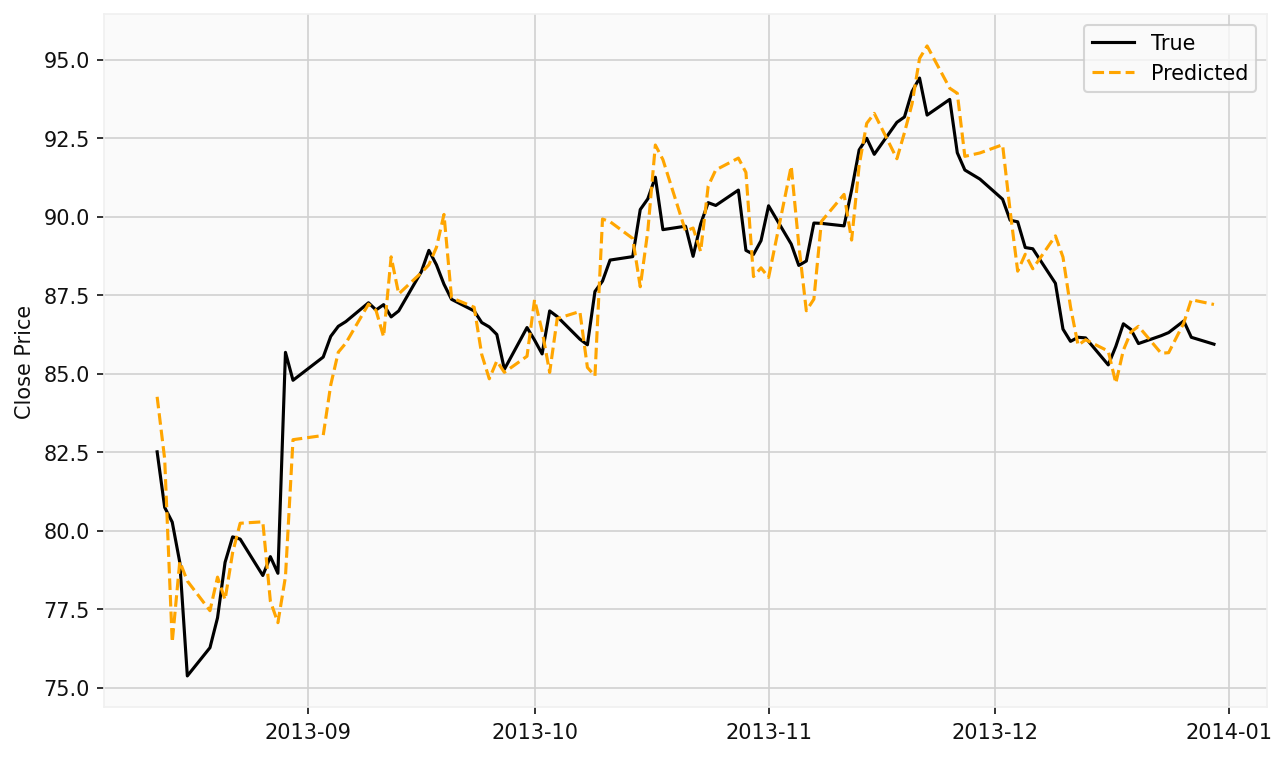
\includegraphics[width=\textwidth]{../images/rnn_prediction.png}
    \caption{RNN}
    \label{fig:rnn_prediction}
  \end{subfigure}
  \begin{subfigure}[b]{0.48\textwidth}
    \centering
    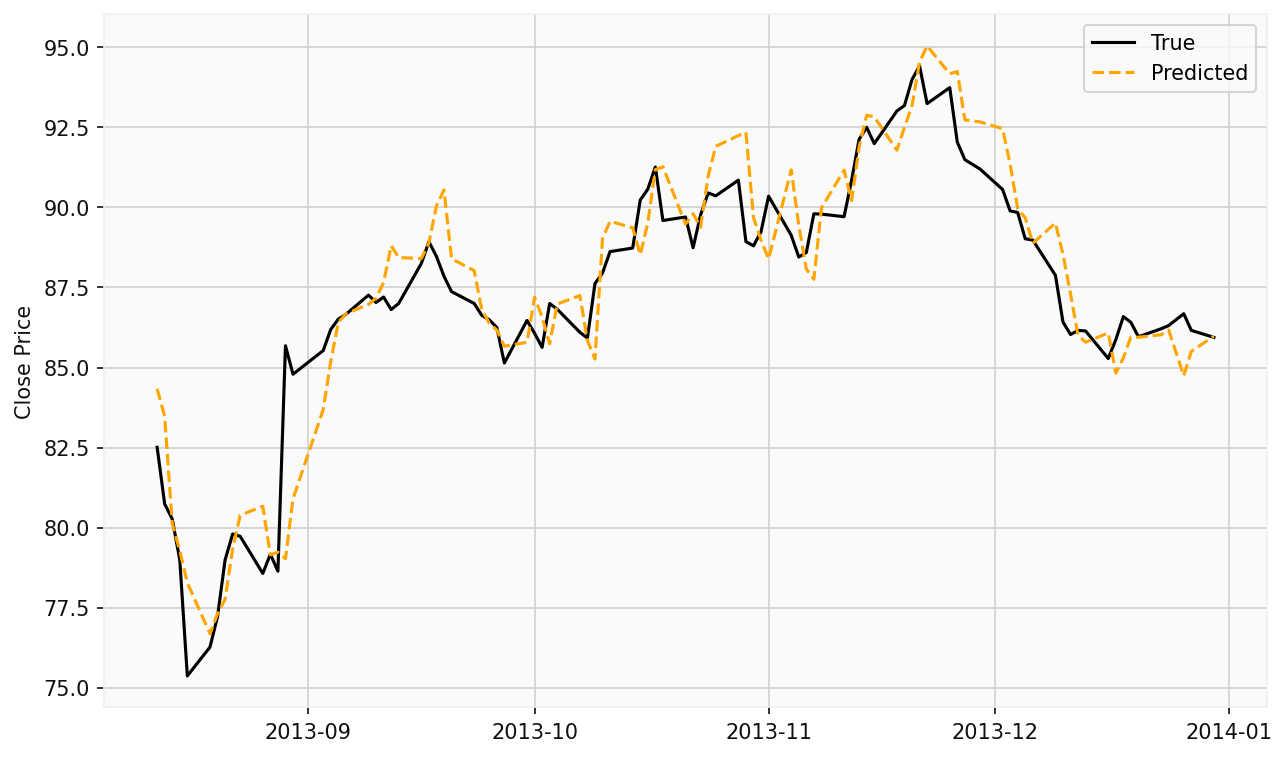
\includegraphics[width=\textwidth]{../images/lstm_prediction.png}
    \caption{LSTM}
    \label{fig:lstm_prediction}
  \end{subfigure}
  \begin{subfigure}[b]{0.48\textwidth}
    \centering
    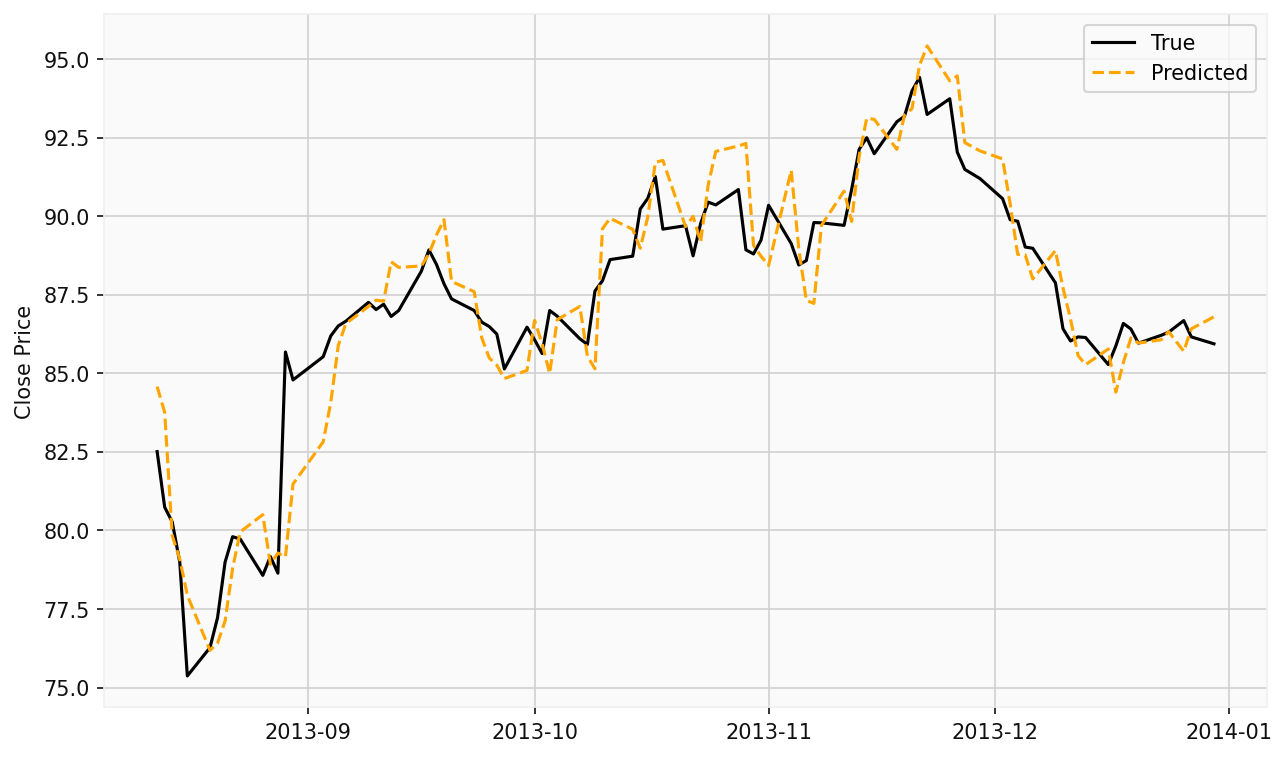
\includegraphics[width=\textwidth]{../images/gru_prediction.png}
    \caption{GRU}
    \label{fig:gru_prediction}
  \end{subfigure}
  \caption{predcitions on the test set (dotted line) of Moving Average Model, RNN, LSTM and GRU}
  \label{fig:predictions}
\end{figure}

\section{Discussion}

In economics there is the theory of efficient markets that states that all publically know factors considering a stock are already priced in, in the stock price and therefore the future value of a stock does not follow any predictable pattern. If there was such a pattern, whoever finds it, would abuse the pattern to make money and in the process destroy the pattern through the stock transactions themselves. Since we only use publically known past prices for our prediction it is not surprising that the last day's Close value seems to be the best prediction for the next day.
Also having such limited data (less than 500 datapoints) in the train set does not help the model to detect such a pattern if there was one. Our models seem to overfit the data quite quickly, meaning they pick up on noise in the train set. Their predictions on the test set are, as we saw, worse than if one would just have taken the last Close value.
Maybe using more datapoints could help to bring out the qualities of recurrent neural networks. One strategy would be to use not daily but secondly stock prices to predict movements even within days. In this way we could easily have more than 10.000 times as many datapoints, if we had stock data for every second instead of every day.

\end{document}
